\chapter[Teoría de Acopladores Direccionales]{Teoría de Acopladores Direccionales} \label{cp:introduction}

Los acopladores direccionales son componentes pasivos de microondas de cuatro puertos utilizados para la división o combinación de potencia entre distintas ramas de un sistema de radiofrecuencia. A diferencia de un divisor de potencia convencional, un acoplador direccional distribuye la señal de entrada de manera desigual y direccional entre sus puertos de salida, propiedad que resulta de particular utilidad para muestrear una fracción controlada de la potencia de una señal sin interrumpir su trayectoria principal.

La Figura~\ref{fig:directional_coupler} muestra los dos símbolos comúnmente utilizados para representar un acoplador direccional, junto con la convención de numeración de puertos empleada a lo largo de este capítulo. Tomando al puerto 1 como puerto de entrada, la mayor parte de la potencia incidente se transmite hacia el puerto 2, denominado \textit{puerto de paso} (\textit{through port}), mientras que una fracción menor y controlada de dicha potencia se transfiere al puerto 3, denominado \textit{puerto acoplado} (\textit{coupled port}). El puerto 4, denominado \textit{puerto aislado} (\textit{isolated port}), no recibe potencia alguna en un acoplador ideal.

\begin{figure}[b!]
    \centering
    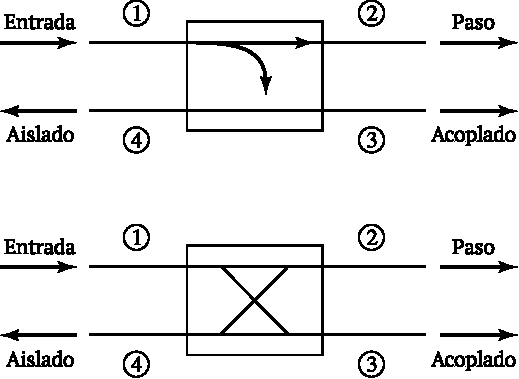
\includegraphics[width=0.7\textwidth]{Figures/Figura_7_4.pdf}
    \caption{Dos símbolos comúnmente utilizados para acopladores direccionales.}
    \label{fig:directional_coupler}
\end{figure}

Esta asignación de puertos, sin embargo, no es fija, sino que depende de cuál de los cuatro puertos se utilice como entrada. Si en cambio la señal se inyecta por el puerto 4, la potencia se reparte entre los mismos puertos 2 y 3, mientras que el puerto que queda aislado es el puerto 1. Es decir, los puertos 1 y 4 resultan mutuamente aislados entre sí, cualquiera sea cuál de los dos se emplee como entrada, mientras que ambos entregan potencia a los puertos 2 y 3, si bien el rol de puerto de paso y puerto acoplado se intercambia entre estos según cuál de los dos primeros se haya excitado. De manera análoga, si la señal se inyecta por el puerto 2 o por el puerto 3, la potencia se reparte entre los puertos 1 y 4, resultando el puerto 3 o el puerto 2, respectivamente, el puerto aislado en cada caso. Esta simetría, presente en todo acoplador direccional ideal, no es una propiedad incidental del dispositivo, sino que constituye la única solución posible cuando una red de cuatro puertos satisface simultáneamente tres condiciones: que sea recíproca, que se encuentre adaptada en cada uno de sus puertos y que no presente pérdidas. La sección siguiente formaliza estas tres condiciones en términos de la matriz de parámetros $S$ de la red, y deriva a partir de ellas la forma general que debe adoptar dicha matriz para dar lugar al comportamiento descripto.

\section{Fundamentos de Acopladores Direccionales}

Por recíproca se entiende una red donde $S_{ij} = S_{ji}$, siendo $i \neq j$. Adicionalmente, si la red se encuentra adaptada en cada puerto, sus coeficientes de reflexión propios son nulos, es decir $S_{11} = S_{22} = S_{33} = S_{44} = 0$, por lo que la matriz de parámetros $S$ puede expresarse como

\begin{equation}
    [S] = 
    \begin{bmatrix} 
        0      & S_{12}   & S_{13}   & S_{14} \\ 
        S_{12} & 0        & S_{23}   & S_{24} \\ 
        S_{13} & S_{23}   & 0        & S_{34} \\ 
        S_{14} & S_{24}   & S_{34}   & 0 
    \end{bmatrix}
\label{eq:ideal_matrix1}
\end{equation}

Puede demostrarse que, para una red sin pérdidas, su matriz de parámetros $S$ debe ser unitaria \cite[p.~145]{pozar2011}, lo cual implica que el producto matricial entre la matriz $S$ transpuesta y la matriz $S$ conjugada debe ser igual a la matriz identidad. Dado que la reciprocidad ya establece que la transpuesta de la ecuación~\eqref{eq:ideal_matrix1} es idéntica a la propia matriz, esta condición se reduce a

\vspace{-0.5cm}
\begin{equation}
    [S]\times[S]^* = [U] 
\label{eq:sin_perdidas}
\end{equation}

donde $[U]$ es la matriz identidad. Siguiendo el desarrollo de \cite[Cap.~7]{pozar2011}, se lleva a cabo la multiplicación definida en la ecuación~\eqref{eq:sin_perdidas}, obteniendo una serie de ecuaciones presentadas a continuación. Del producto entre la fila 2 y la columna 1, y de la fila 3 por la columna 4, se obtiene

\vspace{-1cm}
\begin{subequations}
    \begin{align}
        S_{13}^*S_{23} + S_{14}^*S_{24} = 0 \\
        S_{14}^*S_{13} + S_{24}^*S_{23} = 0
    \end{align}
    \label{eq:eqs_f2c1}
\end{subequations}
\vspace{-0.5cm}

Multiplicando ambas ecuaciones por $S_{24}^*$ y $S_{13}^*$ respectivamente, y restando entre sí las expresiones resultantes, se llega a

\vspace{-0.5cm}
\begin{equation}
    S_{14}^*\,(\lvert S_{13} \rvert^2 - \lvert S_{24} \rvert^2)=0
\label{eq:producto1}
\end{equation}

Realizando el mismo procedimiento para el producto entre la fila 3 y la columna 1, y entre la fila 2 y la columna 4, se obtiene

\vspace{-0.5cm}
\begin{equation}
    S_{23}^*\,( \lvert S_{12} \rvert^2 - \lvert S_{34} \rvert^2)=0
\label{eq:producto2}
\end{equation}

donde una solución posible para las ecuaciones~\eqref{eq:producto1} y \eqref{eq:producto2} es que $S_{14}=S_{23}=0$.

Del resto del producto matricial, correspondiente a la diagonal unitaria, se derivan las siguientes ecuaciones

\begin{subequations}
    \begin{align}
        \lvert S_{12} \rvert^2 + \lvert S_{13} \rvert^2 = 1 \\
        \lvert S_{12} \rvert^2 + \lvert S_{24} \rvert^2 = 1 \\
        \lvert S_{13} \rvert^2 + \lvert S_{34} \rvert^2 = 1 \\
        \lvert S_{24} \rvert^2 + \lvert S_{34} \rvert^2 = 1
    \end{align}
    \label{eq:eqs_lossless}
\end{subequations}
\vspace{-0.5cm}

de las cuales se deduce que $\lvert S_{13} \rvert = \lvert S_{24} \rvert$ y $\lvert S_{12} \rvert = \lvert S_{34} \rvert$. Dado que se trata de números complejos, esta relación solo vincula los módulos de dichos parámetros, sin definir aún sus fases. Se elige arbitrariamente $S_{12}=S_{34}=\alpha$, es decir, dos complejos iguales con fase $0^\circ$, y $S_{13}=\beta e^{j\theta}$ y $S_{24}=\beta e^{j\phi}$, complejos de igual magnitud cuyas fases son constantes pero distinto valor. Para respetar la conservación de energía deben seguir cumpliéndose las ecuaciones~\eqref{eq:eqs_lossless}, de donde resulta $\alpha^2 + \beta^2 = 1$. Multiplicando la fila 2 por la columna 3 se obtiene una ecuación adicional que relaciona los cuatro parámetros $S$ involucrados:

\begin{equation}
    S_{12}^* S_{13} + S_{24}^* S_{34} = 0
\label{eq:producto3}
\end{equation}

Reemplazando por los valores propuestos:

\vspace{-0.5cm}
\begin{subequations}
    \begin{align}
        \alpha\beta e^{j\theta} + \alpha\beta e^{-j\phi} = 0         \\
        e^{j\theta} = -e^{-j\phi} = e^{-j\phi}e^{j\pi}e^{\pm j2n\pi} \\
        \theta + \phi = \pi \pm 2n\pi
    \end{align}
    \label{eq:phase_eqs}
\end{subequations}
\vspace{-0.5cm}

Considerando $n=0$ y con las referencias de fase apropiadas, las dos formas prácticas más comunes son $\theta=\phi=\pi/2$, conocida como acoplador simétrico, y $\theta=0$ y $\phi=\pi$, denominada acoplador antisimétrico. Las matrices de parámetros dispersión correspondientes a estos dos casos son:

\begin{table}[H]
    \centering
    \begin{tabular}{cc}
        \begin{minipage}{0.4\textwidth}
            \begin{equation}
            [S] = \begin{bmatrix}
            0      & \alpha & j\beta & 0      \\
            \alpha & 0      & 0      & j\beta \\
            j\beta & 0      & 0      & \alpha \\
            0      & j\beta & \alpha & 0
            \end{bmatrix}
            \end{equation}
        \vspace{0.5cm}
        \centering
        \textbf{Acoplador simétrico (90º)}
        \end{minipage} &
        
        \begin{minipage}{0.4\textwidth}
            \begin{equation}
            [S] = \begin{bmatrix}
            0      & \alpha & \beta  & 0      \\
            \alpha & 0      & 0      & -\beta \\
            \beta  & 0      & 0      & \alpha \\
            0      & -\beta & \alpha & 0
            \end{bmatrix}
            \end{equation}
        \vspace{0.5cm}
        \centering
        \textbf{Acoplador antisimétrico (180°)}
        \end{minipage}
    \end{tabular}
\end{table}

\vspace{-0.5cm}

donde $\alpha$ es el coeficiente de \textit{paso} de tensión y $\beta$ el coeficiente de \textit{acoplamiento} de tensión. Retomando la convención de puertos presentada en la Figura~\ref{fig:directional_coupler}, la potencia suministrada al puerto 1 se acopla al puerto 3 con el factor de acoplamiento $|S_{13}|^2 = \beta^2$, mientras que el resto de la potencia de entrada se entrega al puerto 2 con el coeficiente $|S_{12}|^2 = \alpha^2 = 1 - \beta^2$, quedando el puerto 4 idealmente aislado.

Los siguientes parámetros se utilizan comúnmente para caracterizar un acoplador direccional:
\begingroup
    \allowdisplaybreaks
    \begin{align}
        \textbf{Acoplamiento} \quad C &= 10 \log \frac{P_1}{P_3} = -20 \log \beta \text{ dB}, \label{eq:coupling} \\
        \textbf{Directividad} \quad D &= 10 \log \frac{P_3}{P_4} = 20 \log \frac{\beta}{|S_{14}|} \text{ dB}, \label{eq:directivity} \\
        \textbf{Aislación} \quad I &= 10 \log \frac{P_1}{P_4} = -20 \log |S_{14}| \text{ dB}, \label{eq:isolation} \\
        \textbf{Pérdidas de inserción} \quad L &= 10 \log \frac{P_1}{P_2} = -20 \log |S_{12}| \text{ dB}. \label{eq:insertion_loss}
    \end{align}
\endgroup

El factor de acoplamiento indica la fracción de la potencia de entrada que se acopla al puerto de salida. La directividad es una medida de la capacidad del acoplador para aislar ondas directas e inversas (o los puertos acoplado y no acoplado). La aislación es una medida de la potencia entregada al puerto no acoplado. Estas cantidades están relacionadas como

\begin{equation}
    I = D + C \text{ dB}. \label{eq:relation}
\end{equation}

Las pérdidas de inserción representan la potencia de entrada entregada al puerto de paso, disminuida por la potencia entregada a los puertos acoplado y aislado. El acoplador ideal tiene directividad y aislación infinitas ($S_{14} = 0$). Entonces, tanto $\alpha$ como $\beta$ pueden determinarse a partir del factor de acoplamiento, $C$.

\section{Acopladores híbridos}
Los acopladores híbridos son casos especiales de acopladores direccionales, donde el factor de acoplamiento es de 3 dB, lo que implica que $\alpha = \beta = 1/\sqrt{2}$. Existen dos tipos de híbridos. El \textit{híbrido en cuadratura} tiene un desfase de 90° entre los puertos 2 y 3 ($\theta = \phi = \pi/2$) cuando se alimenta por el puerto 1, y es un ejemplo de acoplador simétrico. Su matriz de dispersión tiene la siguiente forma:

\begin{equation}
    [S] = \frac{1}{\sqrt{2}} 
    \begin{bmatrix} 
        0 & 1 & j & 0 \\ 
        1 & 0 & 0 & j \\ 
        j & 0 & 0 & 1 \\ 
        0 & j & 1 & 0 
    \end{bmatrix}
    \label{eq:quadrature_hybrid}
\end{equation}

El \textit{híbrido magic-T} y el \textit{híbrido rat-race} tienen una diferencia de fase de 180° entre los puertos 2 y 3 cuando se alimentan por el puerto 4, y son ejemplos de acoplador antisimétrico. Su matriz de dispersión tiene la siguiente forma:

\begin{equation}
    [S] = \frac{1}{\sqrt{2}} 
    \begin{bmatrix} 
        0 & 1  & 1 & 0  \\ 
        1 & 0  & 0 & -1 \\ 
        1 & 0  & 0 & 1  \\ 
        0 & -1 & 1 & 0 
    \end{bmatrix}
    \label{eq:antisymmetric_hybrid}
\end{equation}

\section{Híbrido en Cuadratura (90°)}
Los híbridos en cuadratura son acopladores direccionales de 3~dB con una diferencia de fase de 90° en las salidas de los brazos de paso y acoplado. Este tipo de híbrido se fabrica a menudo en forma de línea microstrip o stripline como se muestra en la Figura~\ref{fig:branch_line_geometry} y también se conoce como \textit{híbrido de línea ramificada}. Otros acopladores de 3~dB, como los acopladores de líneas acopladas o los acopladores Lange, también pueden usarse como acopladores en cuadratura; estos componentes se discutirán en secciones posteriores. Aquí analizaremos la operación del híbrido en cuadratura usando una técnica de descomposición de modo par-impar similar a la utilizada para el divisor de potencia Wilkinson.

Con referencia a la Figura~\ref{fig:branch_line_geometry}, la operación básica del acoplador de línea ramificada es la siguiente. Con todos los puertos adaptados, la potencia que entra al puerto 1 se divide uniformemente entre los puertos 2 y 3, con un desfase de 90° entre estas salidas. No se acopla potencia al puerto 4 (el puerto aislado). La matriz de dispersión tiene la siguiente forma

\begin{equation}
    [S] = \frac{-1}{\sqrt{2}} 
    \begin{bmatrix}
        0 & j & 1 & 0 \\
        j & 0 & 0 & 1 \\
        1 & 0 & 0 & j \\
        0 & 1 & j & 0
    \end{bmatrix}
    \label{eq:quadrature_scattering}
\end{equation}

\begin{figure}[h!]
    \centering
    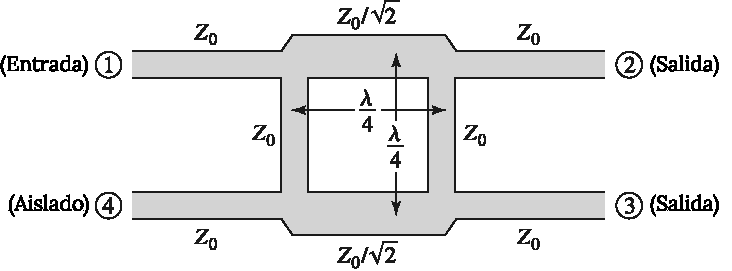
\includegraphics[width=0.9\textwidth]{Figures/Figura_7_21.pdf}
    \caption{Geometría de un acoplador de línea ramificada.}
    \label{fig:branch_line_geometry}
\end{figure}

Obsérvese que el híbrido de línea ramificada tiene un alto grado de simetría, ya que cualquier puerto puede usarse como puerto de entrada. Los puertos de salida siempre estarán en el lado opuesto de la unión respecto al puerto de entrada, y el puerto aislado será el puerto restante del mismo lado que el puerto de entrada. Esta simetría se refleja en la matriz de dispersión, ya que cada fila puede obtenerse como una transposición de la primera fila.

\subsection{Análisis de Modo Par-Impar}
Primero dibujamos el circuito esquemático del acoplador de línea ramificada en forma normalizada, como en la Figura~\ref{fig:branch_line_circuit}, donde se entiende que cada línea representa una línea de transmisión con la impedancia característica indicada normalizada a $Z_0$. El retorno común de tierra para cada línea de transmisión no se muestra. Asumimos que una onda de amplitud unitaria $A_1 = 1$ incide en el puerto 1.

El circuito de la Figura~\ref{fig:branch_line_circuit} puede descomponerse en la superposición de una excitación de modo par y una excitación de modo impar, como se muestra en la Figura~\ref{fig:even_odd_decomposition}. Nótese que la superposición de los dos conjuntos de excitaciones produce la excitación original de la Figura~\ref{fig:branch_line_circuit}, y dado que el circuito es lineal, la respuesta actual (las ondas dispersadas) puede obtenerse de la suma de las respuestas a las excitaciones par e impar.

\begin{figure}[h!]
    \centering
    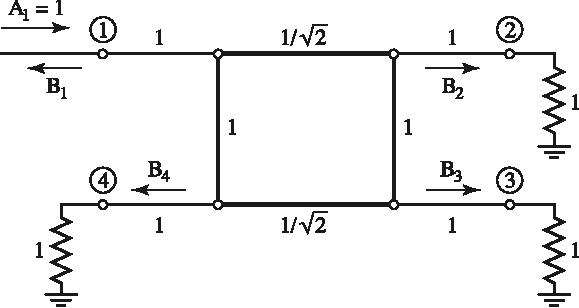
\includegraphics[width=0.6\textwidth]{Figures/Figura_7_22.pdf}
    \caption{Circuito del acoplador híbrido de línea ramificada en forma normalizada.}
    \label{fig:branch_line_circuit}
\end{figure}

Debido a la simetría o antisimetría de la excitación, la red de cuatro puertos puede descomponerse en un conjunto de dos redes desacopladas de dos puertos, como se muestra en la Figura~\ref{fig:even_odd_decomposition}. Debido a que las amplitudes de las ondas incidentes para estos dos puertos son $\pm 1/2$, las amplitudes de la onda emergente en cada puerto del híbrido de línea ramificada pueden expresarse como

\begin{subequations}
    \begin{align}
        B_1 &= \frac{1}{2}\Gamma_e + \frac{1}{2}\Gamma_o, \\
        B_2 &= \frac{1}{2}T_e + \frac{1}{2}T_o, \\
        B_3 &= \frac{1}{2}T_e - \frac{1}{2}T_o, \\
        B_4 &= \frac{1}{2}\Gamma_e - \frac{1}{2}\Gamma_o,
    \end{align}
    \label{eq:scattered_waves}
\end{subequations}


donde $\Gamma_{e,o}$ y $T_{e,o}$ son los coeficientes de reflexión y transmisión de modo par e impar para las redes de dos puertos de la Figura~\ref{fig:even_odd_decomposition}. 

Primero consideremos el cálculo de $\Gamma_e$ y $T_e$ para el circuito de dos puertos de modo par. Esto puede hacerse mejor multiplicando las matrices $ABCD$ de cada componente en cascada en ese circuito, para dar

\begin{equation}
    \begin{bmatrix} 
        A & B \\ 
        C & D 
    \end{bmatrix}_{\!e} =
    \underset{\substack{\text{Derivación} \\ Y=j}}{
        \begin{bmatrix} 
            1 & 0 \\ 
            j & 1 
        \end{bmatrix}
    }
    \underset{\substack{\lambda/4 \\ \text{Línea de} \\ \text{transmisión}}}{
        \begin{bmatrix} 
            0 & j/\sqrt{2} \\ 
            j\sqrt{2} & 0 
        \end{bmatrix}
    }
    \underset{\substack{\text{Derivación} \\ Y=j}}{
        \begin{bmatrix} 
            1 & 0 \\ j & 1 
        \end{bmatrix}
    }
    = \frac{1}{\sqrt{2}} 
    \begin{bmatrix} 
        -1 & j \\ 
        j & -1 
    \end{bmatrix}
    \label{eq:abcd_even}
\end{equation}

\clearpage

\begin{figure}[t]
    \centering
    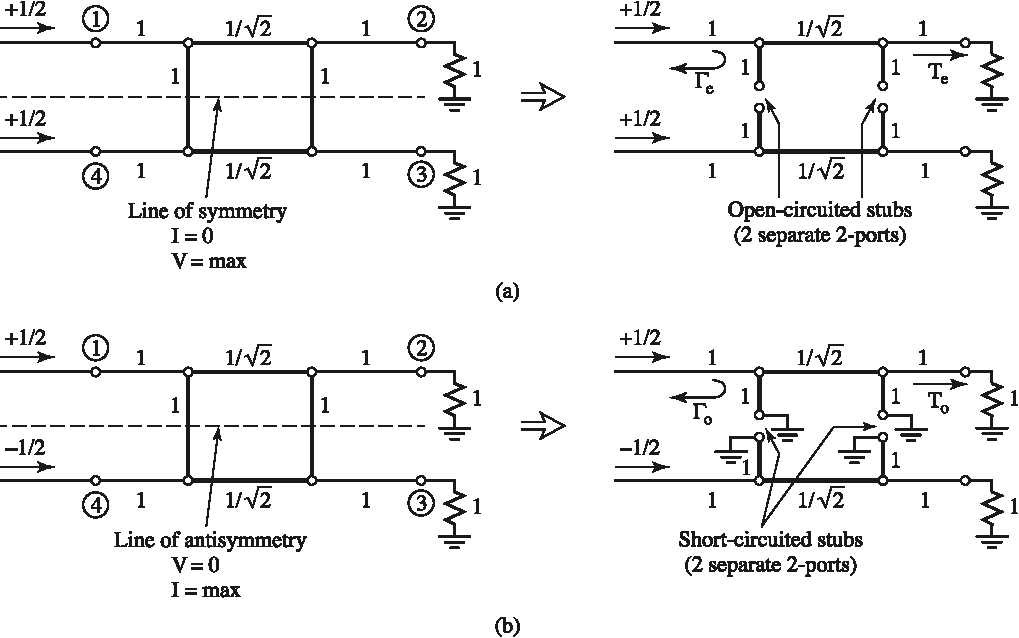
\includegraphics[width=0.9\textwidth]{Figures/Figura_7_23.pdf}
    \caption{Descomposición del acoplador de línea ramificada en excitaciones de modo par e impar. (a) Modo par ($e$). (b) Modo impar ($o$).}
    \label{fig:even_odd_decomposition}
\end{figure}

donde las matrices individuales pueden encontrarse en tablas estándar, y la admitancia de los stubs en derivación de circuito abierto de $\lambda/8$ es $Y = j \tan \beta\ell = j$. Entonces se pueden usar tablas de conversión para convertir de parámetros $ABCD$ (definidos aquí con $Z_o = 1$) a parámetros $S$, que son equivalentes a los coeficientes de reflexión y transmisión. Así

\begin{subequations}
    \begin{align}
        \Gamma_e &= \frac{A+B-C-D}{A+B+C+D} = \frac{(-1+j-j+1)/\sqrt{2}}{(-1+j+j-1)/\sqrt{2}} = 0, \\
        T_e &= \frac{2}{A+B+C+D} = \frac{2}{(-1+j+j-1)/\sqrt{2}} = \frac{-1}{\sqrt{2}}(1+j).
    \end{align}
    \label{eq:even_coefficients}
\end{subequations}

Similarmente, para el modo impar obtenemos

\begin{equation}
    \begin{bmatrix} 
        A & B \\ 
        C & D 
    \end{bmatrix}_{\!o} 
    = \frac{1}{\sqrt{2}} 
    \begin{bmatrix} 
        1 & j \\ 
        j & 1 
    \end{bmatrix}
    \label{eq:abcd_odd}
\end{equation}

lo que da los coeficientes de reflexión y transmisión como

\begin{subequations}
    \begin{align}
        \Gamma_o &= 0, \\
        T_o &= \frac{1}{\sqrt{2}}(1-j).
    \end{align}
    \label{eq:odd_coefficients}
\end{subequations}

Usando las ecuaciones~\eqref{eq:even_coefficients} y~\eqref{eq:odd_coefficients} en~\eqref{eq:scattered_waves} da los siguientes resultados

\begin{subequations}
    \begin{align}
        B_1 &= 0 && \text{(el puerto 1 está adaptado),} \\
        B_2 &= -\frac{j}{\sqrt{2}} && \text{(media potencia, desfase de $-90^{\circ}$ del puerto 1 al 2),} \\
        B_3 &= -\frac{1}{\sqrt{2}} && \text{(media potencia, desfase de $-180^{\circ}$ del puerto 1 al 3),} \\
        B_4 &= 0 && \text{(no hay potencia al puerto 4).}
    \end{align}
    \label{eq:final_results}
\end{subequations}

Estos resultados concuerdan con la primera fila y columna de la matriz de dispersión dada en la ecuación~\eqref{eq:quadrature_scattering}; los elementos restantes pueden encontrarse fácilmente por transposición.

En la práctica, debido al requisito de longitud de cuarto de onda, el ancho de banda de un híbrido de línea ramificada está limitado al 10\%--20\%. Sin embargo, al igual que con los transformadores de adaptación multisección y los acopladores direccionales multiorificio, el ancho de banda de un híbrido de línea ramificada puede aumentarse a una década o más usando múltiples secciones en cascada. Además, el diseño básico puede modificarse para división de potencia desigual y/o diferentes impedancias características en los puertos de salida. Otro punto práctico a tener en cuenta es el hecho de que los efectos de discontinuidad en las uniones del acoplador de línea ramificada pueden requerir que los brazos en derivación se alarguen en 10°--20°.